\section{Experiments}

\subsection{Z-score Versus Activation-score}

Ut est massa, rhoncus sagittis justo vel, cursus interdum odio. Class aptent taciti sociosqu ad litora torquent per conubia nostra, per inceptos himenaeos. Suspendisse elementum pretium sodales. Curabitur ultrices condimentum malesuada. Interdum et malesuada fames ac ante ipsum primis in faucibus. Duis non consectetur nisi, a viverra neque. Vestibulum sodales sed arcu non dictum.

\begin{figure}[h]
\begin{center}
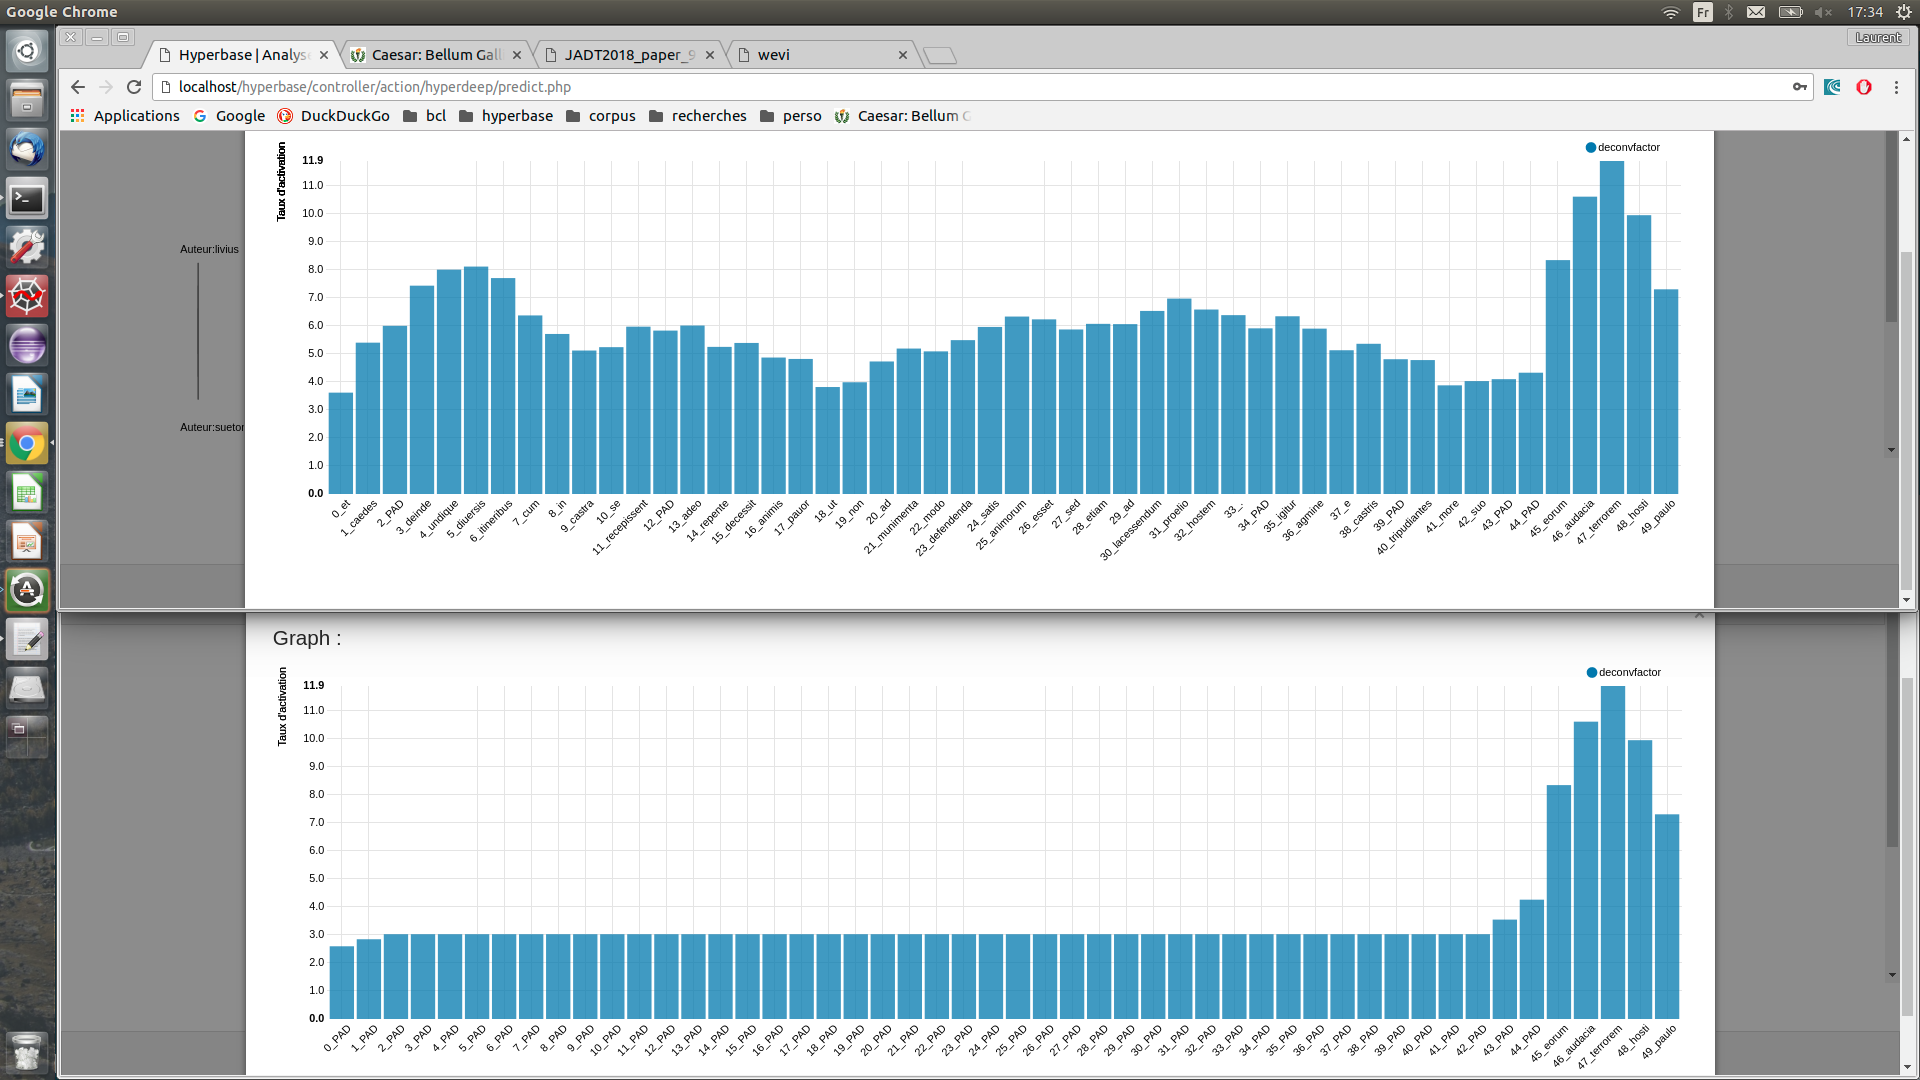
\includegraphics[width=16cm]{img/comaprison.png}
\caption{Z-score Versus Activation-score}
\label{comparision}
\end{center}
\end{figure}

\subsection{Dataset : English}


\subsection{Dataset : French}

" …notre pays advienne, à l'école pour nos enfants, au travail pour l'ensemble de nos concitoyens, pour le climat, pour le quotidien de chacune et chacun d' entre vous. Ces transformations profondes ont commencé et se poursuivront avec la même force, le même rythme, la même intensité"

Cet extrait issu du discours de vœux d'Emmanuel Macron (31 décembre 2017) est mal attribué par l'ADT (Z-score) qui le rapproche statistiquement de De Gaulle, et bien attribué par le Deep learning qui reconnait du Macron.
L'erreur d'attribution statistique s'explique par une phraséologie très gaullienne et la multiplication de marqueurs linguistiques fortement indicés chez de Gaulle : par exemple, de Gaulle avait pour caractéristique de faire des phrases longues et littéraires articulées autour de conjonctions de coordination  comme " et " (z-score = 28 chez de Gaulle, 2 occurrences dans l'extrait). Son discours était également plus conceptuel que la moyenne, et cela se traduisait par une sur-utilisation des articles définis (le, la, l', les) très nombreux dans  l'extrait (7 occurrences) ; particulièrement au féminin singulier (" la " République, " la " liberté, " la " nation ", " la " guerre, etc ; ici " la " même force, " la " même intensité).

Les meilleures performances du deep learning interrogent quant à elle le linguiste et épouse parfaitement ce que l'on sait socio-linguistiquement du discours dynamique de Macron.
La zone d'activation la plus importante de l'extrait concerne le syntagme nominal " transformation profonde ".
Pris séparément, aucun des deux mots du syntagme n'est très macronien d'un point de vue statistique (" transformation " = XXX ; " profonde " = YYY). Mieux : le syntagme lui-même n'est pas attesté dans le corpus d'apprentissage du Président (0 occurrence). 
Cependant, on peut constater que la co-occurrence de " transformation " et de " profonde " s'élève à +XXX chez Macron : ce n'est donc pas l'occurrence d'un mot seul, ou de l'autre, qui est macronienne mais l'apparition simultanée des deux dans une même fenêtre.
Pour autant, la cooccurrence de " transformation " et de " profonde " ne saurait être suffisante pour caractériser Macron, notamment parce que la cooccurrence des deux mots est plus fréquente encore chez Pompidou par exemple ; d'autres indices additionnés sont nécessaires à l'attribution.
Les zones d'activation secondes et complémentaires de l'extrait concernent ainsi les deux verbes " advienne " et " poursuivront ".
D'un point de vue sémantique, les deux verbes conspirent parfaitement, après le syntagme  " transformation profonde ", à donner la dynamique nécessaire à un discours qui prône le changement. Mais c'est les temps verbaux (portés par la morphologie des verbes) qui apparaissent déterminants dans l'analyse.
Le calcul des codes grammaticaux co-occurrents au mot " transformation " indique ainsi que les verbes au subjonctif et les verbes au futur (et également les noms) sont les codes privilégies chez Macron. (GRAPH XXX)
Plus précisément encore, l'algorithme indique que, chez Macron, lorsque " transformation " est associée à un verbe au subjonctif (ici "advienne "), alors il existe le plus souvent un verbe au futur co-présent (ici " poursuivront ").
" Transformation profonde ", " advenir " au subjonctif, " poursuivre " au futur : tous ces éléments signent, ensemble, un discours fait de promesse d'action, dans la bouche d'un président jeune et dynamique.
Enfin, le graphique indique que " transformation " est surtout associée aux noms chez le Président : dans une concentration extraordinaire, l'extrait en recense ainsi 11 ( " pays ", " école ", " enfants ", " travail ", " concitoyens ", " climat ", " quotidien ", " transformations ", " force ", " rythme ", " intensité ").


\subsection{Dataset : Latin}

